\section{级数的极限}
\label{sec:ru-series}
\label{sec:analysis-series}

有限和可以逐项相加，无限多项却无法“加完”。上一节的数列极限提供了处理办法：把前$N$项的和看成一个数列，再问$N$无限增大时它是否趋向确定的数。
本节先用部分和定义级数及其和，计算几类可作基准的级数；随后建立收敛判别，区分不依赖抵消的绝对收敛与依赖抵消的条件收敛；最后说明改变求和次序或合并相邻项会怎样影响结果。

\subsection{部分和、余项与基本级数}
\label{sec:ru-partial-sums}
\label{sec:analysis-series-definition}

给定数列$(a_n)_{n\geq1}$，称$s_N=\sum_{n=1}^Na_n$为第$N$个\term{部分和}（partial sum）。符号\term{无穷级数}（infinite series）$\sum_{n=1}^\infty a_n$描述这一求和过程；
若部分和数列$(s_N)$有有限极限$s$，称级数收敛，并记$\sum_{n=1}^\infty a_n=s$，称$s$为级数的和；否则称级数发散。
三个对象要分清：单项$a_n$、部分和$s_N$与级数的和$s$。例如$a_n=2^{-n}\to0$，而$s_N=1-2^{-N}\to1$。

由$a_N=s_N-s_{N-1}$及差的极限法则，级数收敛必须有$a_N\to0$。反向不成立：上一节末尾的例子说明调和级数$\sum1/n$的单项趋于零，部分和却不是柯西数列，因而发散。

级数是否收敛与前有限项无关，因为删去前$m$项只让部分和相差固定的$s_m$。级数收敛时，$r_N=s-s_N=\sum_{n>N}a_n$称为\term{余项}（remainder），它衡量截断到第$N$项的误差，并且$r_N\to0$。

\paragraph{基准级数}
几何级数与裂项级数的部分和可以直接写出，因而能算出级数的和与余项。由上一章的有限几何和，$|r|<1$时$r^{N+1}\to0$，于是
\begin{equation}
 \sum_{n=0}^\infty r^n=\frac1{1-r},\qquad \Bigl|\sum_{n=N+1}^\infty r^n\Bigr|=\frac{|r|^{N+1}}{|1-r|}.
 \label{eq:analysis-geometric-series}
\end{equation}
$|r|\geq1$时$|r^n|\geq1$，单项不趋零，级数发散。若$a_n=b_n-b_{n+1}$，裂项公式给出$s_N=b_1-b_{N+1}$，所以级数收敛当且仅当$(b_n)$有有限极限。

例如$\sum_{n=1}^\infty\frac1{n(n+1)}=1$，截断到第$N$项的余项恰为$1/(N+1)$。几何级数的余项按公比的幂衰减，裂项级数的余项按$1/N$衰减，后面比较其他级数时，这两种速度都会用到。

若所有$a_n\geq0$，部分和单调不减，由单调有界收敛定理，级数收敛当且仅当部分和有上界；无上界时部分和趋于$+\infty$。
因此对非负项级数统一记
\[
 \sum_{n=1}^\infty a_n=\sup_N\sum_{n=1}^Na_n\in[0,+\infty],
\]
称为非负项级数的扩展总和。总和为$+\infty$时仍称级数发散，但这个记号总有意义，后面比较、重排非负项时可以先在$[0,+\infty]$中比较总和。

\paragraph{$p$级数}
单调性给出了判断$p$级数$\sum_{n=1}^\infty n^{-p}$的办法。设$p>0$，按$n=2^k,\ldots,2^{k+1}-1$分块，每块有$2^k$项，块内每项介于$(2^{k+1})^{-p}$与$(2^k)^{-p}$之间，于是
\[
 2^{-p}\,2^{k(1-p)}\leq\sum_{n=2^k}^{2^{k+1}-1}n^{-p}\leq2^{k(1-p)}.
\]
任一部分和$s_N$都不超过前若干整块之和，所以只需估计整块。

$p>1$时右侧是公比$2^{1-p}<1$的几何级数，每个部分和都不超过$1/(1-2^{1-p})$，级数收敛；
$0<p\leq1$时每块至少为$2^{-p}$，累计任意多块便无界，级数发散；$p\leq0$时单项不趋零。
所以$p$级数恰在$p>1$时收敛，特别地，调和级数发散。这一论证只比较有限个区块，不需要积分判别法。

\subsection{级数极限存在的判别}
\label{sec:ru-series-tests}
\label{sec:analysis-series-tests}

判断级数收敛，就是判断部分和是否有有限极限。非负项的部分和单调，可以用已知级数的上界控制；出现正负项后，还须区分绝对值累计有限与依靠抵消才收敛这两种情形。

\begin{theorem}[正项级数的比较判别]
\label{thm:ru-series-comparison}
设充分大的$n$都有$0\leq a_n\leq b_n$。若$\sum b_n$收敛，则$\sum a_n$收敛；若$\sum a_n$发散，则$\sum b_n$发散。
若$a_n,b_n>0$且$a_n/b_n\to c\in(0,+\infty)$，则两级数同时收敛或同时发散。
\end{theorem}
\begin{proof}
第一句来自非负部分和的单调性：$\sum a_n$的部分和被$\sum b_n$的部分和控制，有限个前项不影响结论。
第二句称为极限比较判别：最终有$(c/2)b_n\leq a_n\leq(3c/2)b_n$，再用第一句。
\end{proof}
例如$\frac{1}{n^2+n}\leq\frac1{n^2}$，而$\frac{2n+1}{n^3}$与$\frac1{n^2}$之比趋于$2$，两者都收敛。

比较判别要求先找到合适的基准。用几何级数作基准，可以得到只看单项本身的判别法。设$a_n>0$。
\begin{theorem}[比值判别与根值判别]
\label{thm:ru-ratio-root-tests}
若$a_{n+1}/a_n\to q$，则$q<1$时$\sum a_n$收敛，$q>1$时发散。若$\limsup a_n^{1/n}=q$，结论相同。
\end{theorem}
\begin{proof}
比值情形：$q<1$时取$q<\rho<1$，充分靠后有$a_{n+1}\leq\rho a_n$，逐次代入得$a_{N+j}\leq a_N\rho^j$，与几何级数比较即收敛；$q>1$时充分靠后的项递增，不趋于零，级数发散。
根值情形：$q<1$时取$q<\rho<1$，由上极限的定义，充分靠后的尾部上确界小于$\rho$，于是$a_n<\rho^n$，与几何级数比较；$q>1$时有无穷多个$n$使$a_n^{1/n}>1$，即$a_n>1$，单项不趋零。
\end{proof}
两种判别在$q=1$时都没有结论：$\sum1/n$发散而$\sum1/n^2$收敛，它们的比值和$n$次根都趋于$1$。这时只能回到比较等更精细的方法。
以上判别都要求各项非负；对一般级数，可以先把它们用于$\sum|a_n|$。

\paragraph{绝对收敛与条件收敛}
若$\sum|a_n|$收敛，称$\sum a_n$\term{绝对收敛}（absolute convergence）。它的意思是：即使不依赖正负抵消，各项的绝对贡献之和也有限。
\begin{theorem}[绝对收敛蕴含收敛]
\label{thm:ru-absolute-convergence}
若$\sum|a_n|$收敛，则$\sum a_n$收敛，其和$s$满足$|s-s_N|\leq\sum_{n>N}|a_n|$。
\end{theorem}
\begin{proof}
对$m>n$，
\[
 |s_m-s_n|\leq\sum_{k=n+1}^m|a_k|\leq\sum_{k>n}|a_k|,
\]
右侧是收敛非负级数的余项，与$m$无关且随$n$增大趋于零，所以$(s_n)$满足柯西准则。令$m\to\infty$即得误差界。
\end{proof}
例如$\sum(-1)^{n+1}/n^2$由$p=2$的情形绝对收敛，截断到第$N$项的误差不超过$\sum_{n>N}1/n^2\leq\sum_{n>N}\frac1{n(n-1)}=\frac1N$。

若原级数收敛，而$\sum|a_n|$发散，称为\term{条件收敛}（conditional convergence）。这需要同时证明两件事；只知道绝对值级数发散，不能排除原级数也发散。
最基本的依靠抵消而收敛的情形是交错级数。
\begin{theorem}[交错级数的Leibniz判别]
\label{thm:ru-leibniz}
若$b_n\geq0$单调不增且$b_n\to0$，则$\sum_{n=1}^\infty(-1)^{n+1}b_n$收敛，其和$s$满足$|s-s_N|\leq b_{N+1}$。
\end{theorem}
\begin{proof}
偶数部分和$s_{2n+2}=s_{2n}+(b_{2n+1}-b_{2n+2})$单调不减，奇数部分和$s_{2n+1}=s_{2n-1}-(b_{2n}-b_{2n+1})$单调不增，并且每个偶数部分和都不超过任何奇数部分和。
所以两列分别有界单调，各自收敛；它们之差$s_{2n+1}-s_{2n}=b_{2n+1}\to0$，两个极限相同，记为$s$。给定误差后，奇偶两类下标的尾部分别满足要求，取较晚的起点即知$s_N\to s$。
$s$位于任意一对相邻部分和$s_N,s_{N+1}$之间，因此$|s-s_N|\leq|s_{N+1}-s_N|=b_{N+1}$。
\end{proof}
例如交错调和级数$\sum(-1)^{n+1}/n$收敛，绝对值级数却是调和级数，所以它条件收敛。若$\sum b_n$本身收敛，Leibniz条件给出的交错级数则是绝对收敛的，不能一概称为条件收敛。
图~\ref{fig:analysis-process-series-terms-sums}并排比较调和级数与交错调和级数：两者的项都趋于零，累计后的行为却不同。

\begin{figure*}[!htbp]
 \centering
 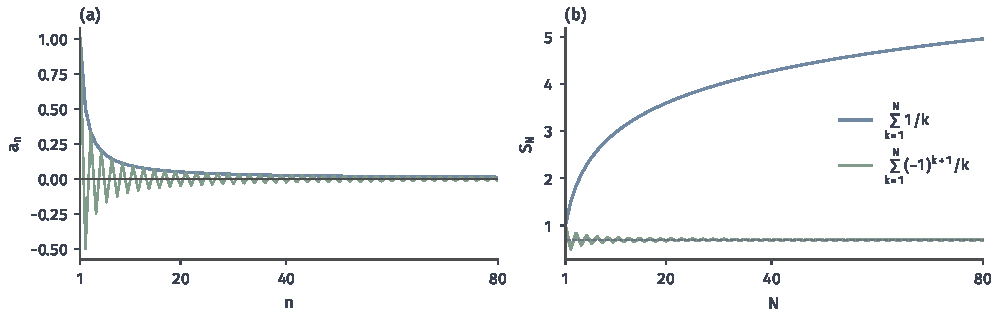
\includegraphics[width=169.0mm]{figures/01-mathematical-preliminaries-upper/00-shared/matplotlib/chapter3-concept-processes/series-terms-sums.pdf}
 \caption{(a) 蓝、绿折线分别连接$1/n$与$(-1)^{n+1}/n$的前80项。(b) 对应的部分和：调和部分和继续增长，交错调和部分和趋于虚线所示的$\log2$。项趋零只是级数收敛的必要条件；图展示有限段，收敛或发散由正文中的判别证明。}
 \label{fig:analysis-process-series-terms-sums}
\end{figure*}

\paragraph{Dirichlet判别}
交错级数的论证可以推广：若一列数的部分和有界振荡，再配上单调趋零的权重，乘积级数仍收敛。这一推广称为Dirichlet判别，作为补充推导列在这里，第~\ref{sec:ru-power-series-uniform}节证明幂级数在端点附近的一致收敛时要用到同样的技巧。

设$A_N=\sum_{n=1}^Na_n$满足$|A_N|\leq M$，$b_n\geq0$单调趋零。对$m\leq k$记$A^{(m)}_k=\sum_{n=m}^ka_n$，则$|A^{(m)}_k|\leq2M$，约定$A^{(m)}_{m-1}=0$。
把$a_k=A^{(m)}_k-A^{(m)}_{k-1}$代入有限和并重新组合（称为有限分部求和），得到
\[
 \sum_{k=m}^Na_kb_k=A^{(m)}_Nb_N+\sum_{k=m}^{N-1}A^{(m)}_k(b_k-b_{k+1}).
\]
由于$b_k-b_{k+1}\geq0$，右侧绝对值不超过$2M\bigl[b_N+\sum_{k=m}^{N-1}(b_k-b_{k+1})\bigr]=2Mb_m$，它与$N$无关且随$m$增大趋于零，由柯西准则知$\sum a_nb_n$收敛。
取$a_n=(-1)^{n+1}$便回到交错情形。

\subsection{级数的重排与分组对收敛的影响}
\label{sec:ru-series-rearrangement-grouping}
\label{sec:analysis-series-rearrangement-grouping}

有限和可以任意交换项的先后、任意加括号。无穷级数的和是部分和的极限，改变次序或加括号会改变部分和数列，因而需要重新检验。
重排改变各项进入累计的顺序，分组只把原次序中有限个相邻项合并，两种操作的效果不同。

\paragraph{级数的重排}
若$\pi:\{1,2,\ldots\}\to\{1,2,\ldots\}$为双射，级数$\sum_na_{\pi(n)}$称为原级数的\term{重排}（rearrangement），它恰好使用每一项一次。
\begin{theorem}[保持和的重排]
\label{thm:ru-rearrangement}
非负项级数的任意重排与原级数有相同的扩展总和；绝对收敛级数的任意重排仍收敛，并且和不变。
\end{theorem}
\begin{proof}
对非负项，重排的每个部分和只含有限个原下标，它们都不超过某个$N$，所以该部分和不超过$s_N$，从而不超过原扩展总和；反过来，原来的前$N$项也全部出现在重排的某个有限前段中。两个方向分别取上确界即得。

设原级数绝对收敛，和为$s$，记重排的部分和为$t_K$。给定$\varepsilon>0$，先选$N$使$\sum_{n>N}|a_n|<\varepsilon$，再选$K_0$使$\pi(1),\ldots,\pi(K_0)$已经包含$1,\ldots,N$。
当$K\geq K_0$时，$t_K-s_N$是若干个下标大于$N$的项之和，故$|t_K-s_N|<\varepsilon$；又$|s_N-s|<\varepsilon$，所以$|t_K-s|<2\varepsilon$。
\end{proof}

条件收敛没有这一保证。记前$N$项中正项之和为$P_N$、负项绝对值之和为$Q_N$。若二者的极限有一个有限，由$s_N=P_N-Q_N$收敛可知另一个也有限，
于是$\sum|a_n|$有限，与条件收敛矛盾；所以正项与负项的总和都是$+\infty$。

对任意目标$L$，按原相对次序取正项直到部分和超过$L$，再取负项直到低于$L$，如此反复；若原级数含有零项，每轮再插入一个尚未使用的零项。
正负项的总和都无限，每一轮都在有限步内结束，所有项最终都被用到；而$a_n\to0$使每次越过$L$的幅度趋于零，因此这个重排的和为$L$。
可见条件收敛级数的和依赖抵消的顺序，不能按有限和的交换律任意调换。

\paragraph{级数的分组}
分组保持原项的顺序，只把相邻项合为一项。取$0=n_0<n_1<n_2<\cdots$，令$c_j=\sum_{k=n_{j-1}+1}^{n_j}a_k$，则分组后前$J$项的和恰为$s_{n_J}$，是原部分和的子列。
所以原级数收敛到$s$时，分组后的级数也收敛到$s$，绝对收敛与条件收敛都是如此。
反向不成立：$1-1+1-1+\cdots$的部分和在$1$与$0$之间交替，原级数发散，
按$(1-1)+(1-1)+\cdots$分组后各项却都为零。分组只保留部分截断位置，可能掩盖块内的振荡。

非负项没有这种抵消：原部分和单调，分组截断又越过每一个原截断位置，两者的上确界相同，所以非负项级数可以任意保序分组，即使总和为$+\infty$。
